\section{Black box modeling approach}

% Difference with bottom-up, not the same application, not the same goal
The black-box modeling method works similarly to the bottom-up modeling approach.
It studies the relationship and transfer function between the input and the output of a silicon function.
Unlike the bottom-up method, the model is only build for external inputs and outputs.
It is not meant to be chained with other similar models, using a special chaining method.
Instead, it targets board-level circuit simulations.
The motivation behind this model is related to the \gls{seed} methodology (TODO: REFERENCE).
The goal is to provide a black box model that is fast to simulate and can be distributed without disclosing sensitive intellectual property.

% introduction, failure relation between input and output
The main benefit of this model is to abstract the internal silicon complexity.
The model focuses on describing the failure of an output when an input is stressed.
At board-level, failure criteria can be more easily set from the chip specification.
After setting the failure criteria, the approach is to inject rectangular pulses on an input pin, and record when an output is in fault.

% access to the signals
Since the characterized nets are external pins, they are physically accessible.
Where the bottom-up method was done in simulation, the black box models can be derived from actual measurements.
Overall, the aim of the black-box model is make abstractions of the inner complexity of the chip.

\subsection{Characterization}

% How is the characterization conducted
Once again, a variable width/variable amplitude rectangular pulses are applied on an input pin.
The output pin is then observed to detect at which (width, amplitude) it is going out of specification.

% What is characterized
This characterization is performed on the testchip, on the complete pre-regulator/bandgap/regulator function.
The characterization pulses are injected on the $V_{batt}$ input.
The output pin is $V_{2p5}$, the regulated supply.
It is supposed to deliver a 2.5V regulated supply.
The failure criteria is set at a voltage below 2.1V.
It corresponds to a level below which digital cells powered by this supply will have noise margins too small for proper operation.

% Fig X shows the waveform of the VBAT injected current when stressed with a TLP (square) impulse.
% The TLP waveform before the capacitor is shown for reference.
%TODO: WAVEFORM CURRENT VBAT AND TLP BEFORE INJECTION CAPACITOR ?

% Detail the characterization
The characterization curve is given in Fig. \ref{fig:cz-black-box}.
X-axis is the pulse width, and y-axis is the minimal stress amplitude that caused a failure on the output.

\begin{figure}[!h]
  \centering
  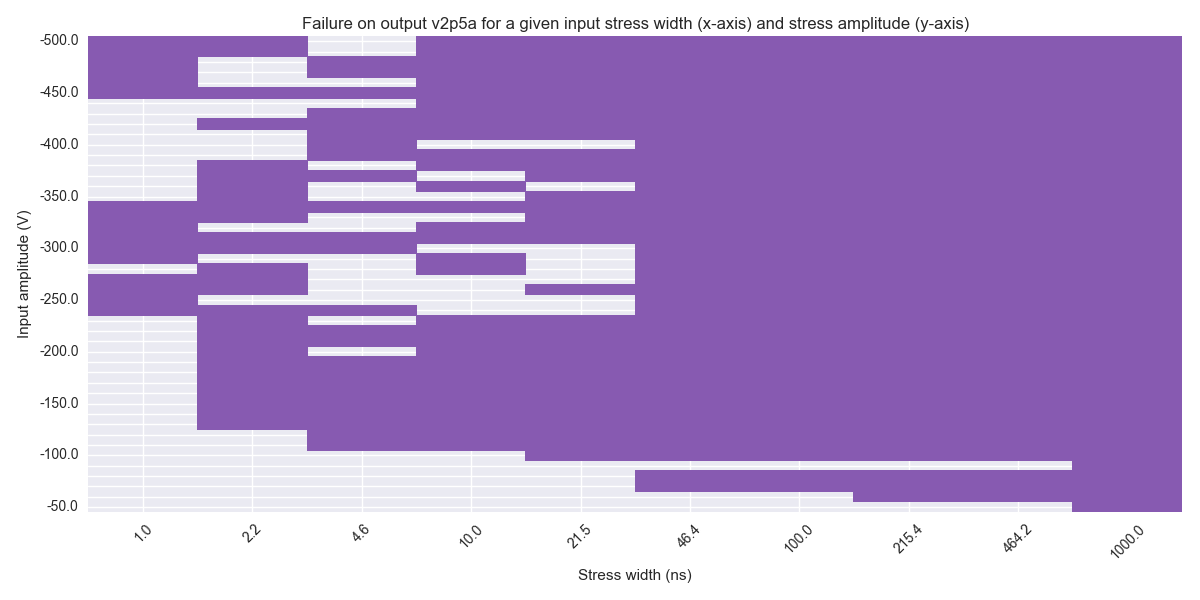
\includegraphics[width=\textwidth]{src/4/figures/black_box_regulator.png}
  \caption{Black-box characterization of the regulation function}
  \label{fig:cz-black-box}
\end{figure}

% What to do with that
The characterization curve is interesting in itself.
%TODO: We that below this value the function is in fail, etc
However, the motivation for this model is to replace the transistor-level schematic inside a SPICE simulation at board-level.
Given a pulse width and an amplitude on $V_{batt}$, the model can estimate the disturbance amplitude and width on $V_{2p5}$.
However, the model itself is not an electrical model, only a failure model.
It cannot determinate, given for instance an input voltage, how much current is flowing into it.
This is also true for the output.
Thus, this method calls for an electrical model of \gls{io}.
The next section details how to solve this issue.

\subsection{Electrical modeling of inputs and outputs}

%TODO: What the hell do I write here...

% Conditions where the model must work
Transient simulations, and in powered-conditions

%

\subsection{Failure modeling}

% Transition with previous section, now possible to do electrical modeling

%
To model the failure, a verilog-ams model is written.
It continuously checks the input current and deduces if the output is going out of spec.

\begin{algorithmic}
- Maintain an array SLICES[] that will contain amount of slices found superior to a voltage
- Record time intervals where voltage is higher than minimum failure voltage
- For each interval:
  - divide it in 1ns slices
  - For each slice:
      - if slice average voltage superior to voltage 1, increment SLICES[1]
      - if slice average voltage superior to voltage 2, increment SLICES[2]
      - etc
      - until slice average voltage no longer superior to voltage n or max voltage reached
- For each entry of SLICES:
  - multiply SLICES[i] by 1ns
  - This translates in : Voltage was superior to voltage 1 for SLICES[i] * 1ns
  - If the point (SLICES[i] * 1ns, voltage 1) is superior than the failure curve, then mark this point as FAIL
\end{algorithmic}

GRAPHS FOR DESCRIBING PRINCIPLE

At the end, list of all fails.

\subsection{Validation in simulation}

SPICE simulation and comparison with transistor level schematic

\subsection{Validation on a ESD Gun stress}
Use it in other simulations (Gun for instance), to check if failure level can be predicted

\subsection{Conclusion on black-box modeling}

Interesting for distributing the models to external parties.
... ?
